\documentclass[14pt]{extarticle}
\usepackage[russian]{babel}
\usepackage[utf8x]{inputenc}
\usepackage{float}
\usepackage{amsmath}
\usepackage{graphicx}
\usepackage{subcaption}
\usepackage[colorinlistoftodos]{todonotes}
\renewcommand{\baselinestretch}{1.5}
\usepackage[left=3cm,right=1cm,top=1.5cm,bottom=2cm]{geometry}
\setlength{\parindent}{0mm}
\setlength{\parskip}{1em}
\usepackage{hyperref}
\usepackage{subfiles}
\hypersetup{
    colorlinks,
    citecolor=black,
    filecolor=black,
    linkcolor=black,
    urlcolor=black
}

\begin{document}

\begin{titlepage}
\subfile{sections/0-titlepage}
\end{titlepage}

\tableofcontents
\newpage 

\section{Введение}
\subfile{sections/1-introduction}
\newpage  

\section{Описание аппаратной части разработанной системы}
\subfile{sections/2-hardware}
\newpage

\section{Описание программного обеспечения}
В рамках данной работы было написано програмное обеспечение для работы с ультразвуковым стетоскопом. Програмное обеспечение написано на языке C\# для платформы Windows.

В функционал програмного обеспечения входит:
\begin{itemize}
  \item Получение сигнала от АЦП ЛА-н10-12USB
  \item Отображение сигнала в реальном времени на экране в виде графика
  \item Отображение спектра сигнала полученного в результате быстрого преобразования Фурье
  \item Отображение скользящего среднего сигнала
  \item Возможность записи сигнала на жесткий диск для последующей обработки
\end{itemize}

\subsection{Инструкция по установке ПО}
\begin{itemize}
  \item Скачать драйверы для АЦП ЛА-н10-12USB по ссылке:\\ \url{http://rudshel.ru/software.html}
  \item Запустить и установить файл \verb|RShUSBDriver_XP_Vista_7_8_x86_x64_SDK2_2.0.x.y.exe| (драйверы для USB устройств)
  \item Запустить и установить файл \verb|RshSDKSetup_2.0.x.y.exe| (средства разработки ПО (SDK))
  \item Скачать проект для работы со стетоскопом по ссылке \url{https://github.com/tandav/ultrasonic-stethoscope/tree/master/Rudshel/forms-timer-label}
  \item Скомпилировать проект с помощью IDE Microsoft Visual Studio.
\end{itemize}

\subsection{Описание интерфейса пользователя ПО} 
\begin{figure}[H]
\centering
% 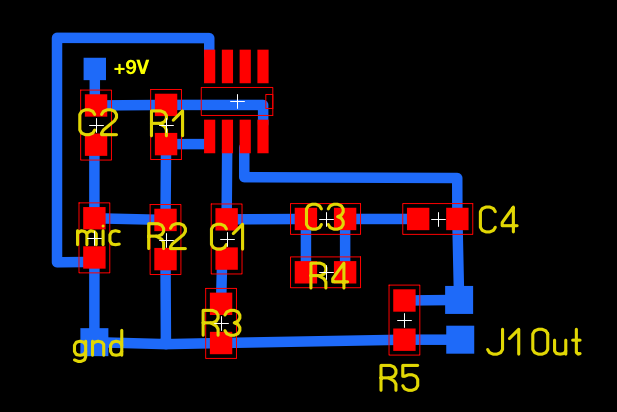
\includegraphics[width=14cm]{sprint-layout-circuit.png}
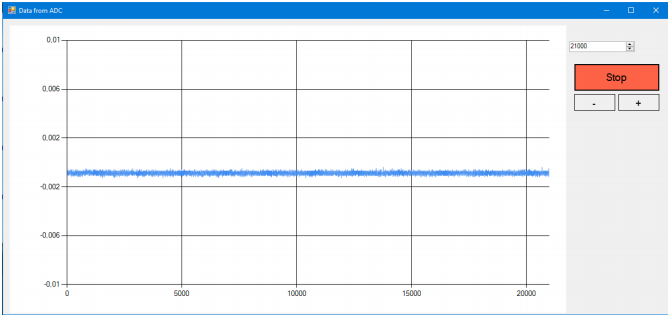
\includegraphics[width=\textwidth]{images/screenshot.png}
\caption{Скриншот работы программы}
\end{figure}
В центре находится график сигнала с АЦП. Справа находится кнопка старт/стоп, которая управлет запуском и остановкой сбора сигнала с АЦП. Справа вверху есть числовое поле, которое отвечает за количество точек по горизонтальной оси на графике. Кнопки "+/-" Отвечают за увеличение и уменьшение размеров графика (zoom).

\subsection{Описание кода программы}
В начале программы задаются параметры размера буффера и частоты дискретизации (\verb|RATE|).
\begin{verbatim}
const uint   BSIZE              = 524288; // размер буффера
const double RATE               = 8.0e+7;
\end{verbatim}

Далее при нажатии пользователем на кнопку старт, программа начинает инициализацию АЦП. Она проверяет подключено ли устройство, проверяет его работоспособность и начинает сбор данных.

За инициализацию отвечают следующие строчки в коде:
\begin{verbatim}
//========================== ИНИЦИАЛИЗАЦИЯ ================        
st = device.EstablishDriverConnection(BOARD_NAME); //загрузка и 
подключение к библиотеке абстракции устройства
if (st != RSH_API.SUCCESS) SayGoodBye(st);
st  = device.Connect(1); //Подключаемся к устройству. Нумерация с 1.
if (st != RSH_API.SUCCESS) SayGoodBye(st);
p.startType           = (uint)RshInitMemory.StartTypeBit.Program; 
//Запуск сбора данных программный. 
p.bufferSize          = BSIZE; //Размер внутреннего блока данных, 
по готовности которого произойдёт прерывание.
p.frequency           = RATE;  //Частота дискретизации.
p.channels[0].control = (uint)RshChannel.ControlBit.Used;  //Сделаем 0-ой канал активным.
p.channels[0].gain    = 10; // коэффициент усиления для 0-го канала. 
[1, 2, 5, 10] ~ [+-0.2V, +- 0.4V, +-1V, +- 2V]
st = device.Init(p); //Инициализация устройства (передача 
выбранных параметров сбора данных)
if (st != RSH_API.SUCCESS) SayGoodBye(st); //После инициализации 
неправильные значения в структуре будут откорректированы.
\end{verbatim}

Далее программа ждет пока пользователь нажмет кнопку старт. При нажатии на кнопку старт вызывается функция \verb|button1_Click|, которая в свою очередь запускает новый процесс \verb|backgroundWorker1_DoWork|. Этот процесс собирает данные с АЦП в бесконечном цикле пока пользователь не нажмет на кнопку стоп. Он записывает значения с АЦП в структуру данных очередь, доступ к которой имеет UI-процесс (процесс, отвечающий за отображение и обработку элементов пользовательского интерфейса). По мере обновления данных UI процесс обновляет график.

За старт, сбор данных и остановку АЦП отвечает следующий блок кода: 

\begin{verbatim}
double[] buffer = new double[p.bufferSize]; //Получаемый из платы буфер.
uint waitTime = 100000; // Время ожидания(в миллисекундах) до наступления прерывания. Прерывание произойдет при полном заполнении буфера.  // default = 100000
while (getting_data)
{
    stopwatch.Restart();

    st = device.Start(); // Запускаем плату на сбор буфера. по идее нужно для каждого буффера start-stop (в цикле for) Но вроде и так работает и так быстрее намного. (Типа старт за циклом, стоп - внутри for; оба за циклом - не работуют)
    if (st != RSH_API.SUCCESS) SayGoodBye(st);

    st = device.Get(RSH_GET.WAIT_BUFFER_READY_EVENT, ref waitTime);
    if (st != RSH_API.SUCCESS) SayGoodBye(st);

    st = device.GetData(buffer); // very big amount of data
    if (st != RSH_API.SUCCESS) SayGoodBye(st);

    device.Stop();

    // Queue Dequeue and Enqueue implementation with arrays
    double[] values_to_draw_copy = (double[])values_to_draw.Clone();
    for (int i = 0; i < x_axis_points - r_buffer_size; i++) 
        values_to_draw[i] = values_to_draw_copy[r_buffer_size + i];

    for (int i = 0; i < r_buffer_size; i++)
        values_to_draw[x_axis_points - r_buffer_size + i] = buffer[BSIZE / r_buffer_size * i];

    stopwatch.Stop();
    Console.WriteLine("GetData() time:\t" + stopwatch.ElapsedMilliseconds + "ms");
} 
\end{verbatim}

Также процесс backgroundWorker замеряет время каждого цикла сбора данных. (stopwatch.Restart() и stopwatch.Stop()) Это время процесс пользовательского интерфейса выводит на экран.

\subsection{Измерение времени работы АЦП}
Как уже было сказано выше, в зависимости от различных значений размера буффера и частоты дискретизации у АЦП уходит различное время на перезапуск и сбор данных. Эти вычисления производились при помощи стандартной функции-секундомера из стандартной библиотеки C\#.

\subsection{Паралельные вычисления в программе}
В программе используются паралельные вычисления. Присутсвуют два потока. Один поток работает с АЦП: принимает данные и записывает во временный буфер. Другой поток - отрисовывает данные из буффера на графике а также обрабатывает команды пользователя. 

Паралельные вычисления используются из-за необходимости непрерывно получать данные с АЦП, чтобы избежать потери данных. Также, если не использовать паралельные вычисления, то приложение может не реагировать на команды пользователя из за того что процессор будет занят работой с АЦП.

\newpage
\section{Заключение}
В процессе данной работы был создан рабочий прототип устройства, позволяющего анализировать в реальном времени звуковой сигнал, поступающий от сердца или легких. Данное устройство может применяться для получения дополнительной информации, которую человек не может услышать на обычном стетоскопе.

Сфера применения не ограничена медициной, устройство позволяет анализировать любые типы ультразвуковых сигналов.

Развитие проекта можно продолжить в направлении улучшения качества звука. Для этого нужно использовать более дорогие микрофон и усилитель. Также нужно произвести опрос врачей о том, какие именно характеристики звука со стетоскопа важны.

Улучшений в програмном обеспечении можно достигнуть путем оптимизации алгоритмов распаралеливания на нескольких ядрах процессора или на видеокарте. На основе информации от докторов, можно сделать систему распознавания различных забовалеваний легких и сердца.

Разработка данного проекта велась с помощью системы контроля версий git. Исходный код програмного обеспечения, этапы создания и документация доступны по адресу:

\url{https://github.com/tandav/ultrasonic-stethoscope}

\newpage
\renewcommand\refname{Ссылки на источники}
\begin{thebibliography}{}
\bibitem{latexcompanion} 
Аналого цифровой преобразователь ЛА-н10-12USB\\
\url{http://www.rudshel.ru/show.php?dev=14}

\bibitem{latexcompanion} 
Драйверы и програмное обеспечение для устройств ЗАО "Руднев-Шиляев"\\
\url{http://rudshel.ru/software.html}

\bibitem{latexcompanion} 
Документация по программированию устройств ЗАО "Руднев-Шиляев"\\
\url{http://www.rudshel.ru/soft/SDK2/Doc/CPP_USER_RU/html/index.html}

\bibitem{latexcompanion} 
Руководство пользователя ЛА-н10-12USB\\
\url{http://www.rudshel.ru/pdf/LA-n10-12USB(y).rar}

\bibitem{latexcompanion} 
Внешний USB АЦП/ЦАП E14-140-M\\
\url{http://www.lcard.ru/products/external/e-140m)}

\bibitem{latexcompanion} 
Схема усилителя для микрофона\\
\url{http://full-chip.net/analogovaya-elektronika/70-usilitel-dlya-elektretnogo-mikrofona-s-nizkim-urovnem-shuma-shema.html}

\bibitem{latexcompanion} 
Руководство пользователя и технические характеристики операционного усилителя MCP6022\\
\url{https://lib.chipdip.ru/291/DOC000291231.pdf}

\bibitem{latexcompanion} 
Исходный код, документация и этапы создания проекта ультразвукового стетоскопа\\
\url{https://github.com/tandav/ultrasonic-stethoscope}

\end{thebibliography}


\end{document}
